%!TEX root = ../pres - final.tex

\section{Speaker Diarization}

\begin{frame}{Speaker Diarization}

\end{frame}

\begin{frame}{Formulación matemática}

\end{frame}

\subsection{Componentes del sistema}
\begin{frame}{Componentes del sistema}{}

\end{frame}

\subsection{Procesamiento acústico}

\begin{frame}{Elminación de ruido / Detección de silencios}
  \begin{center}
    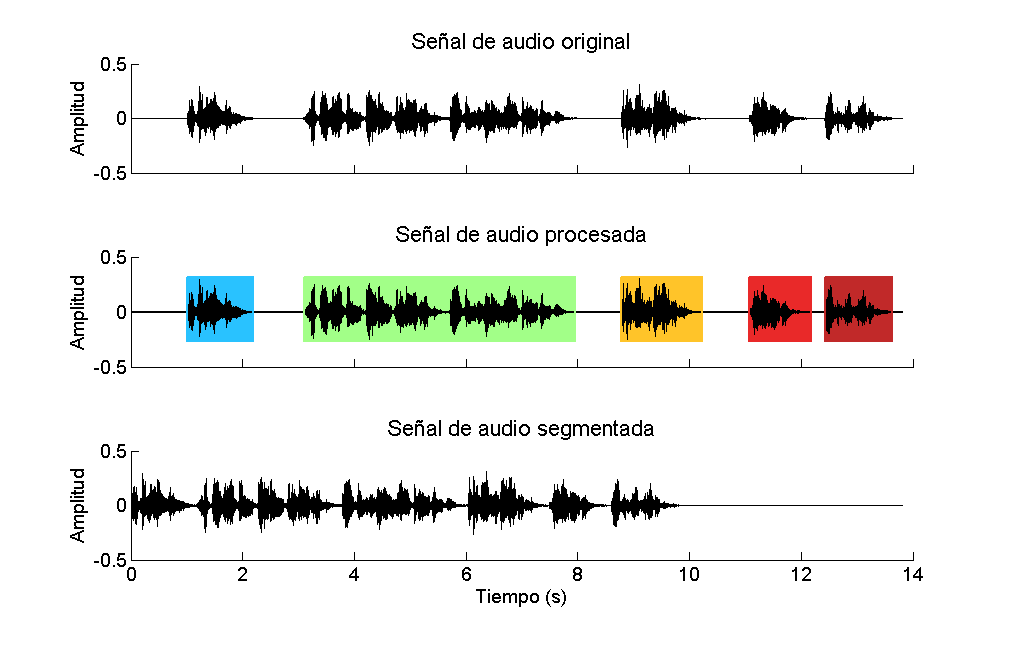
\includegraphics[width=1\textwidth]{gfx/f-silence}
  \end{center}
\end{frame}

%\subsubsection{Obtención de vector de características}

\begin{frame}{Mel Frequency Cepstrum Coefficient}
  \begin{itemize}
    \item \small{FFT (ventana) -> Banco de filtros triangular (Mel Scale) -> Log -> DCT -> MFCC}
  \end{itemize} 
  \begin{center}
    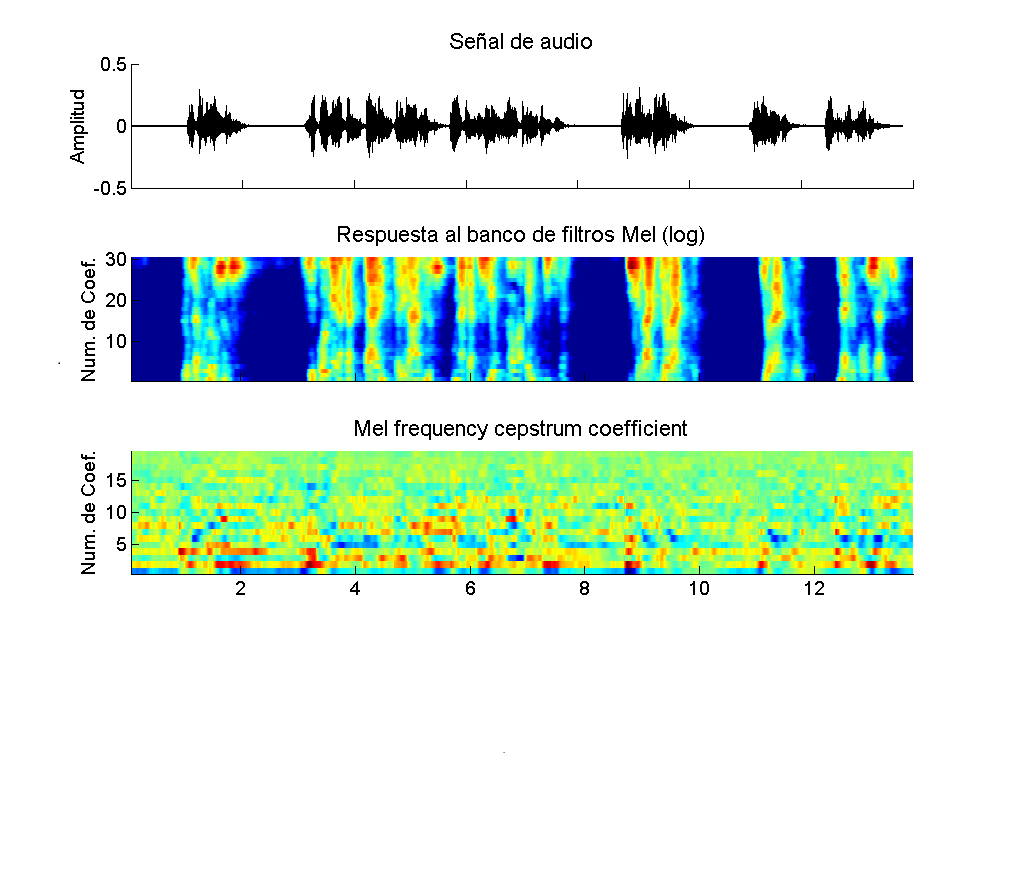
\includegraphics[width=1\textwidth]{gfx/f-mfcc}
  \end{center}
\end{frame}